\section{Forms Module}\label{sec:01}

Forms allow users to perform a daily checkup of the equipment, assigned to them. A new Form items can be added in the "Form Item" folder. Forms functionality is currently under development, but it will contain a Collection of the "Form Items". A User can change the status (Accepted or not) of the Form Item on the Form Class web page. Every Form has the Status property, that can be created and modified in the "Users and Personnel" module.

\subsection{Form Item}
In order for the Item to be shown in he form, it must be created on the Form Item page with the following properties: \textbf{Accepted} and \textbf{Form Type Item}.

    \begin{figure}[!htbp]
    \centering
    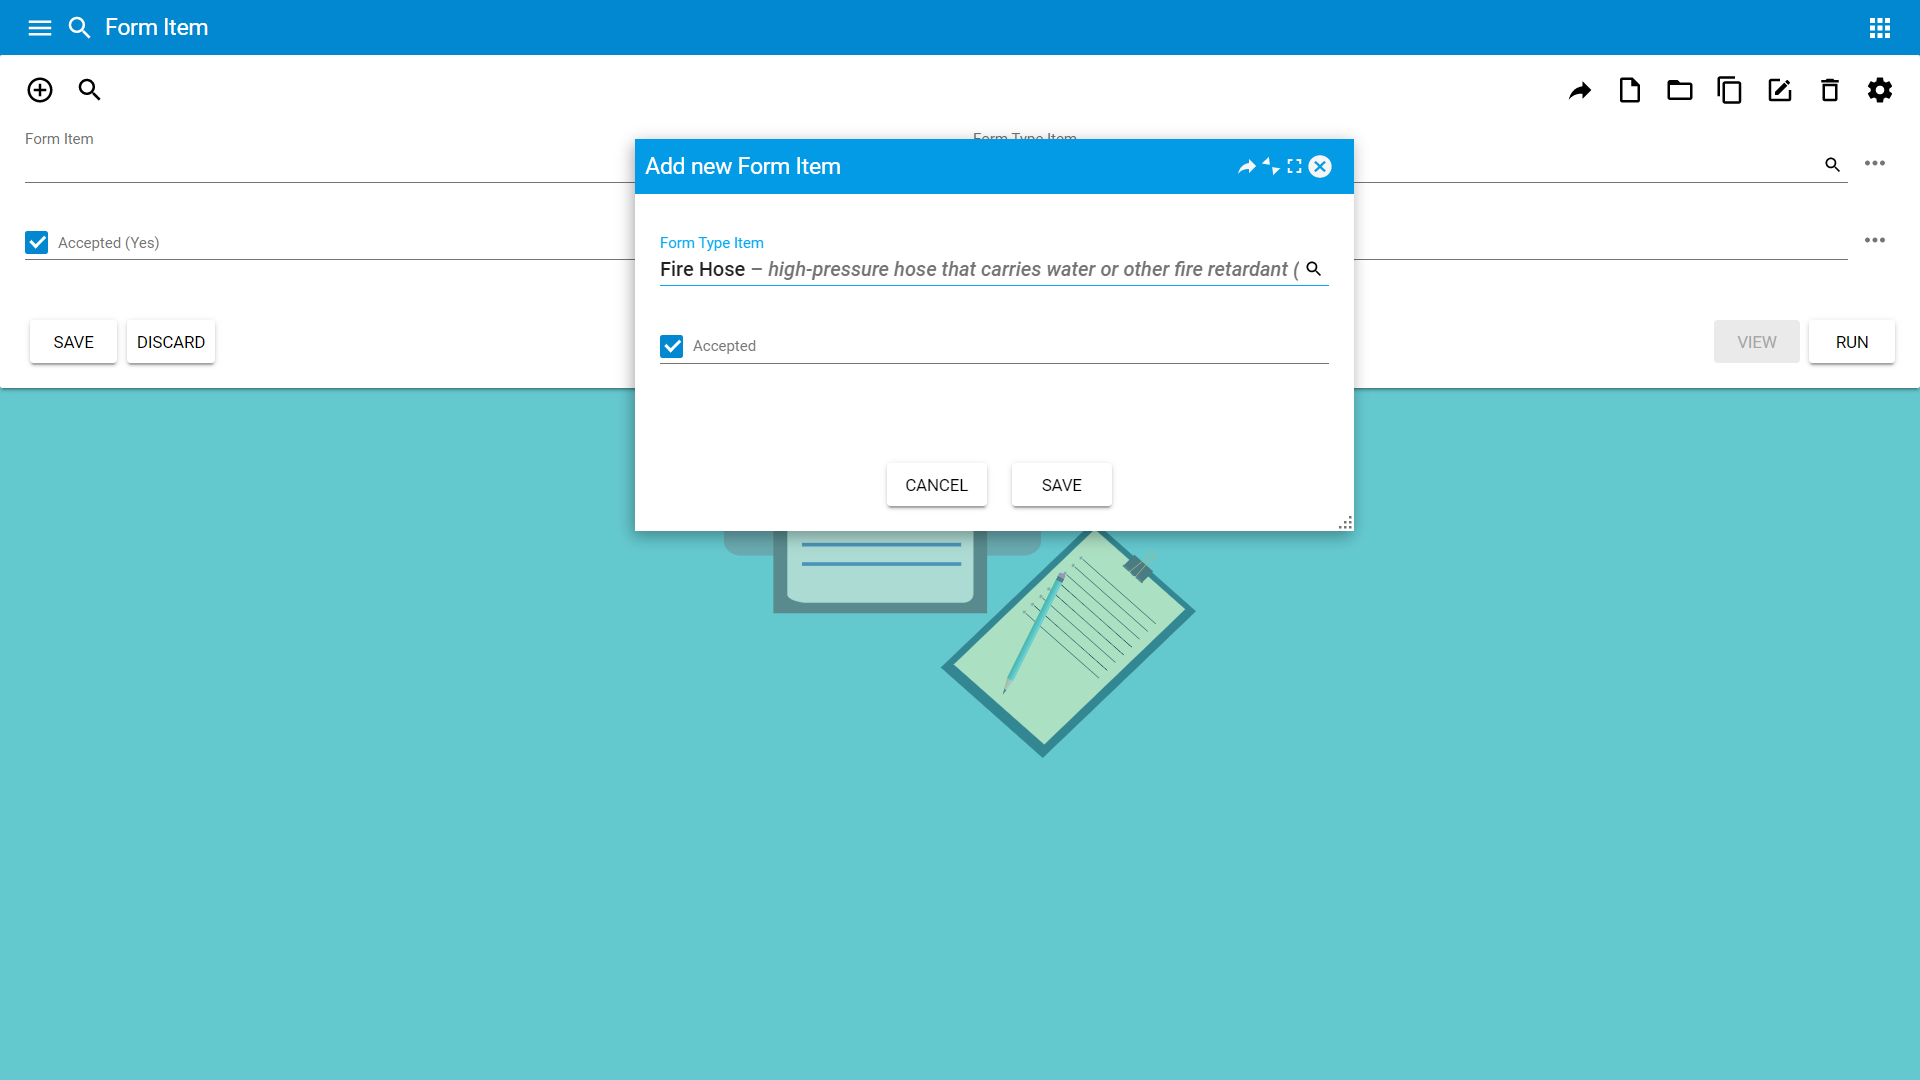
\includegraphics[width=0.95\linewidth]{sections/forms/images/add_new_form_item.png}
    \caption{Form Item creation.}\label{sections/forms/images/add_new_form_item}
    \end{figure}

Users can perform search operation for the form items based on their \textbf{Accepted} status or \textbf{Form Type Item} field.
\newpage

\subsection{Form Type Item}
\textbf{Form Type Item} is a base class for the \textbf{Form Item} creation. Many Form Items can be created from one Form Type Item. 

Form Type Item has the unique Title (without white spaces) and Description fields. For example, a new Form Type Item can be: "\textbf{Title:} \textit{Fire Gloves}; \textbf{Description}: \textit{Important part of the personal protection equipment}."  

% \hyperref[sections/equipment/images/Fig.3]{Fig.~\ref*{sections/equipment/images/Fig.3}}.

    \begin{figure}[!htbp]
	\centering
	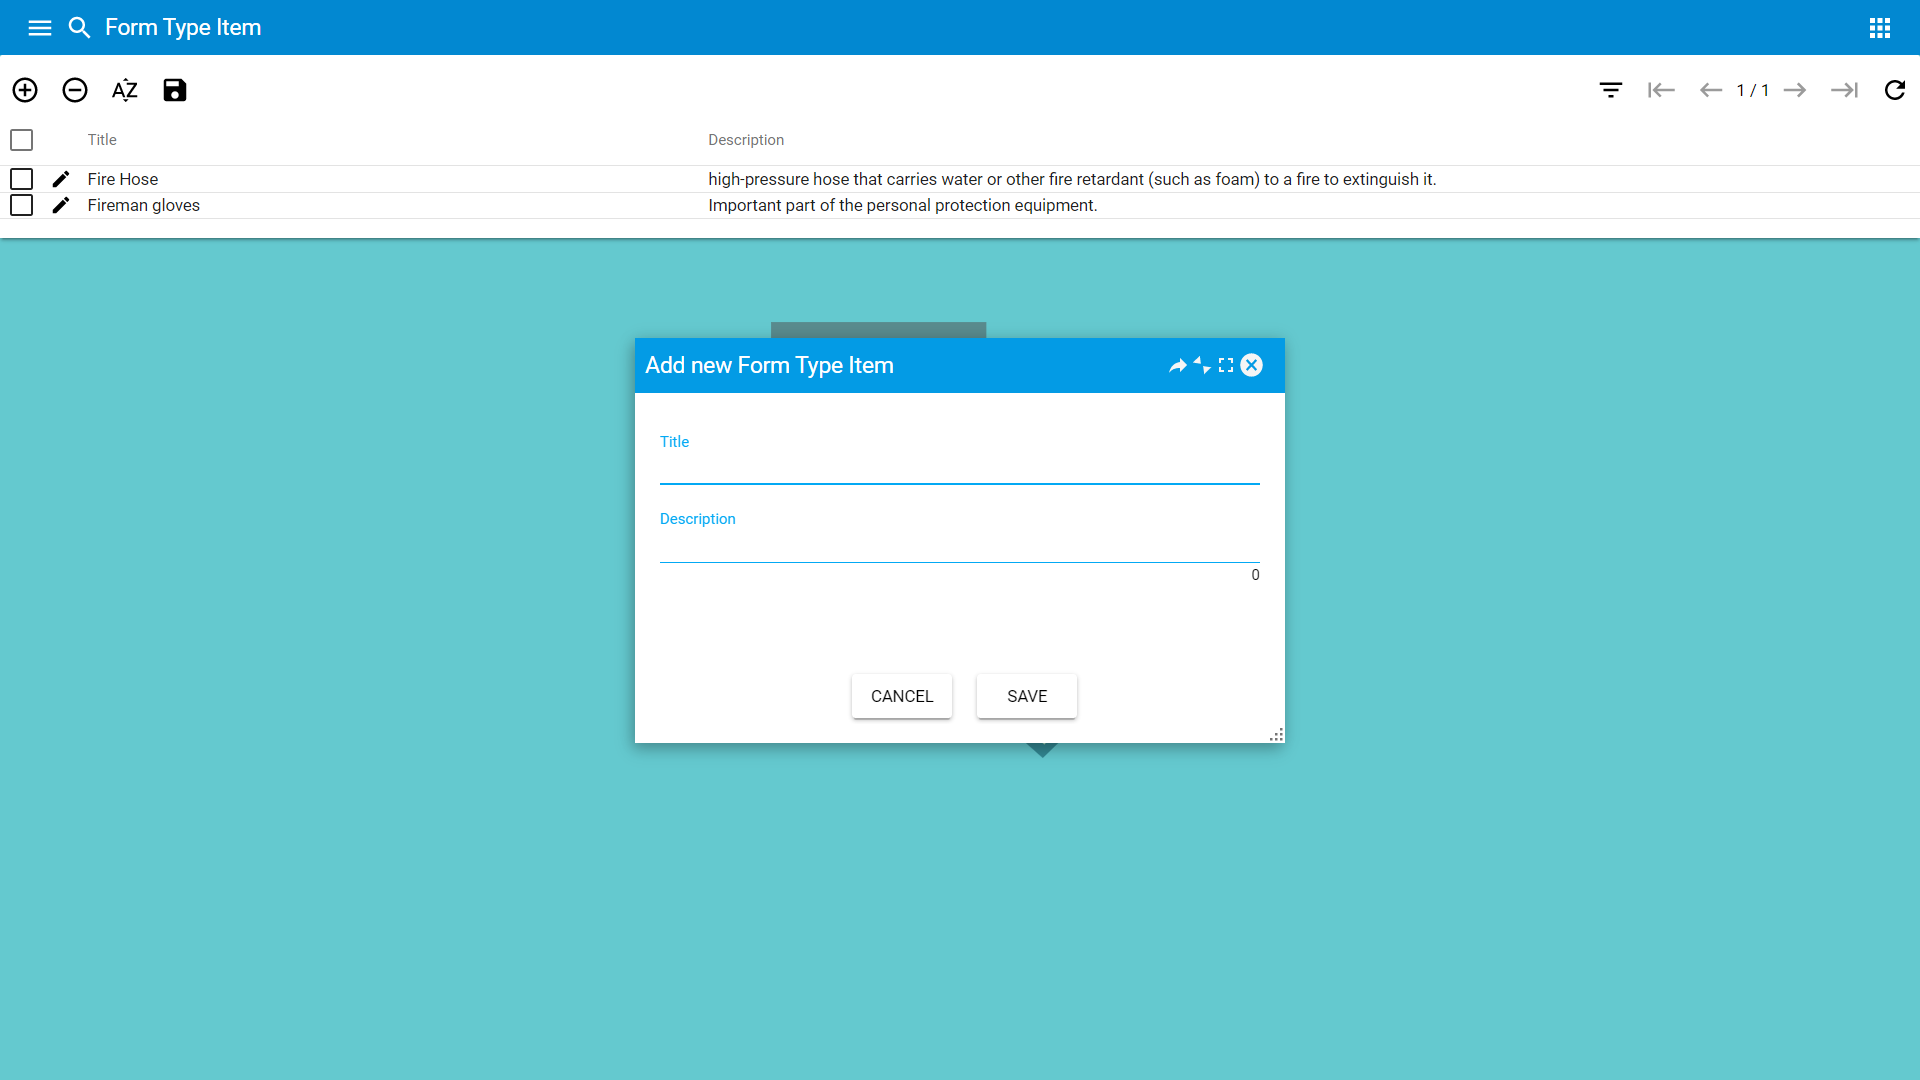
\includegraphics[width=0.95\linewidth]{sections/forms/images/add_newform_type_item.png}
	\caption{Form Type Item creation.}\label{sections/forms/images/add_newform_type_item}
	\end{figure}

Users can perform search operation for the form type items based on their \textbf{Title} or \textbf{Description} values.
\newpage

\subsection{Form Type}
The \textbf{Form Type} is currently under development. 

\textbf{Form Type} is a tool to use the Forms and update the Form Items' statuses. For example, manager Andriy created the Form Type that can be assigned to employee with a specific role, for example Vehicle Driver. Then all the employee with Vehicle Driver role will have the permission to update current form in order to track the status of the equipment during the daily checkup. 

For now, the Form has the unique \textbf{Title} name, \textbf{Assigned Role},  \textbf{Form Class} and \textbf{Description} fields. It is expected that on the next release there will be N additional fields representing status of the Form Items, that can be updated by workers with the specified role.

\begin{figure}[!htbp]
\centering
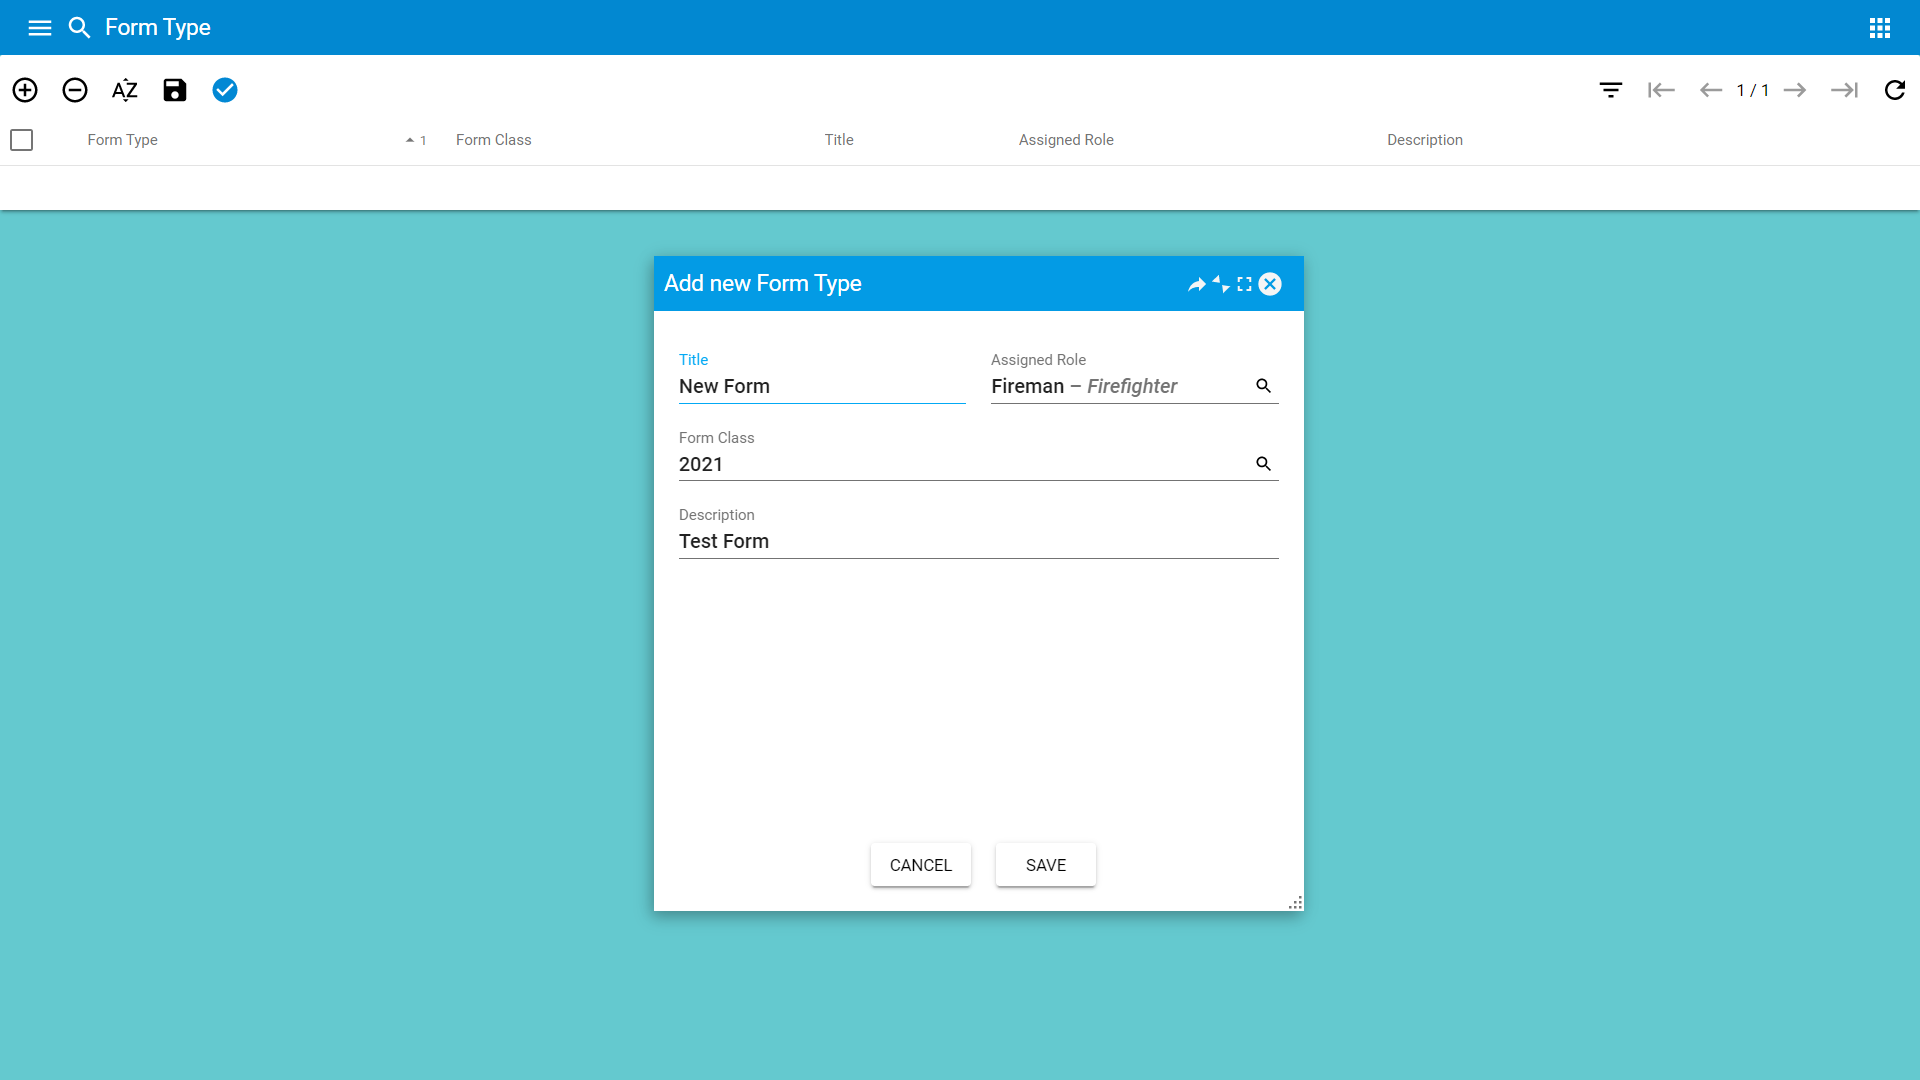
\includegraphics[width=0.95\linewidth]{sections/forms/images/form_type_master.png}
\caption{Form Type creation.}\label{sections/forms/images/form_type_master}
\end{figure}

\newpage
Form Type search query can be used to filter the existing form types, and then to delete or update them. 
\begin{figure}[!htbp]
\centering
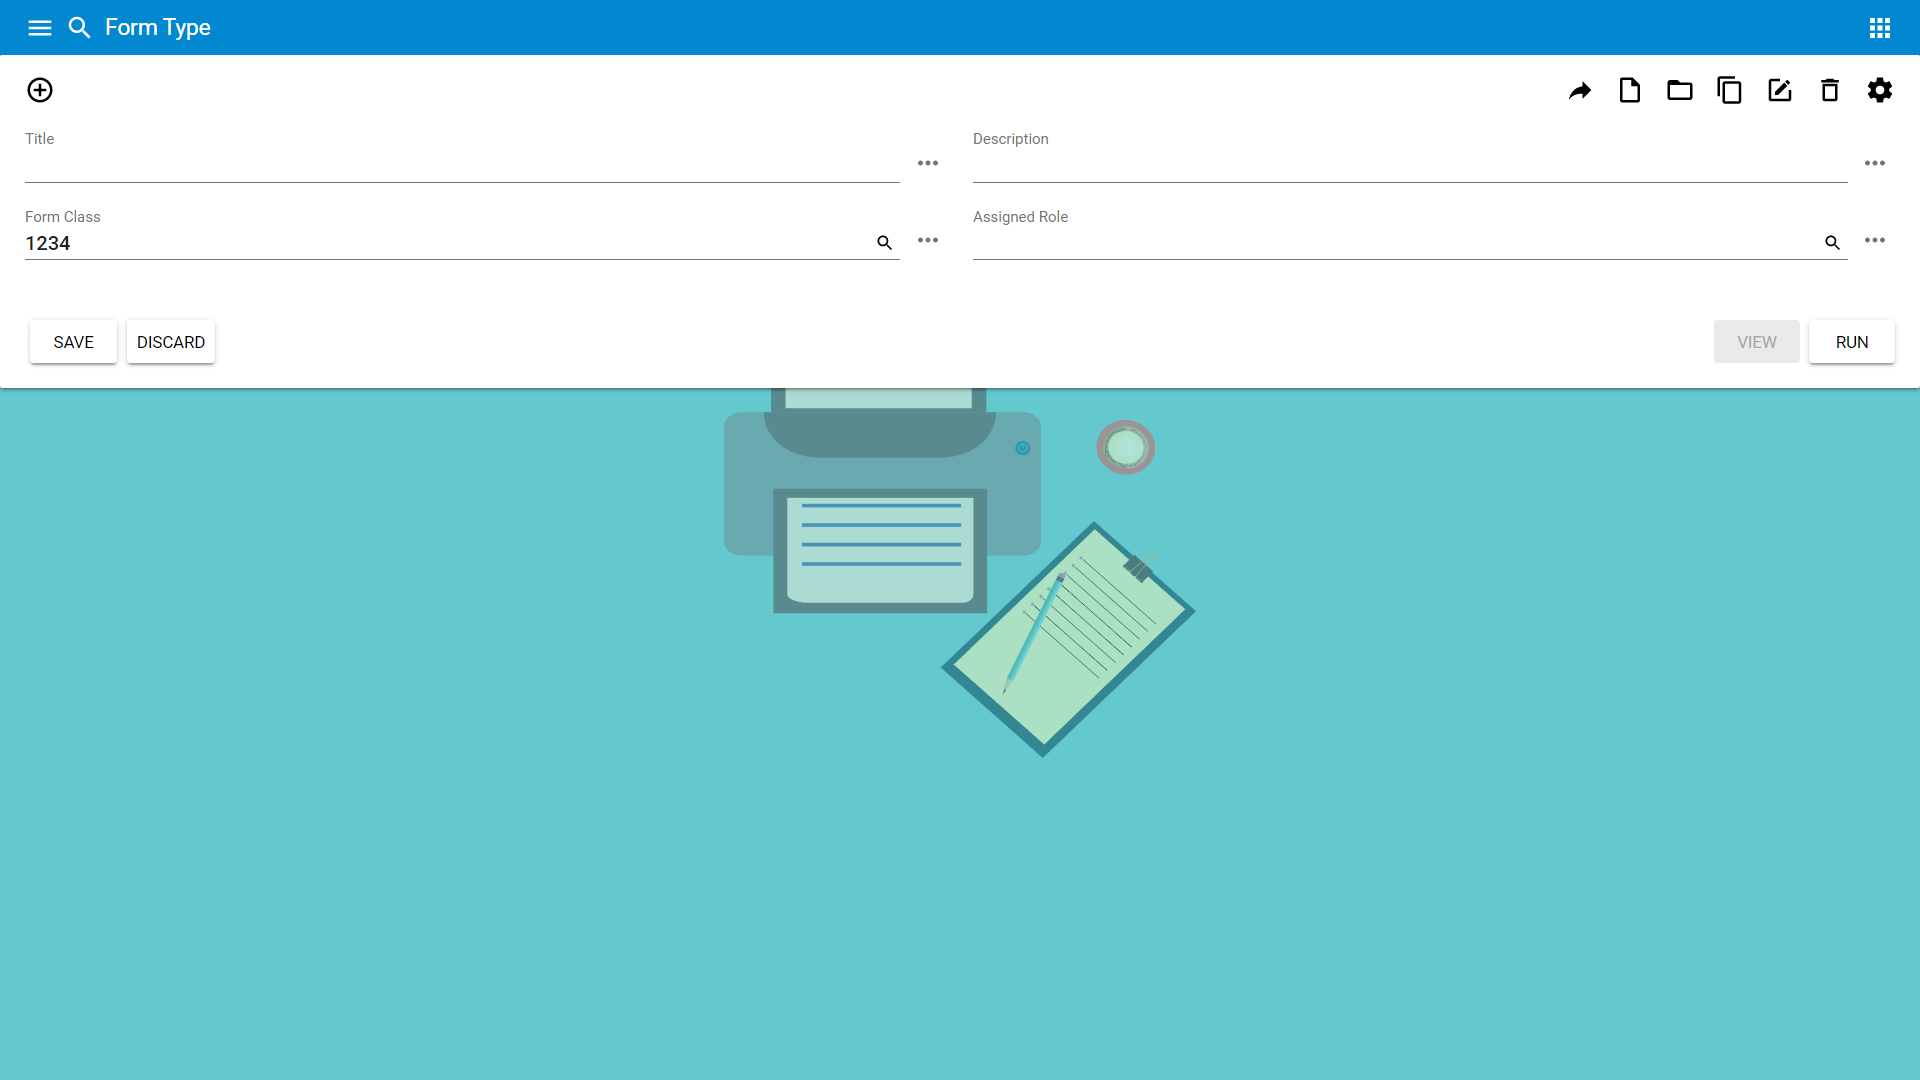
\includegraphics[width=0.95\linewidth]{sections/forms/images/form_type_centre.png}
\caption{Form Type search query.}\label{sections/forms/images/form_type_centre}
\end{figure}

For the next release, it is also planned to correctly fine-tune the BatchUpdate action on the Form Type page. After running the Search query, you can see the checkbox circle on the top of the Form Type page. This is the BatchUpdate action. It updates the status of multiple Form Type entities at once. \textit{You need to select at least one row to perform this action}.

\begin{figure}[!htbp]
\centering
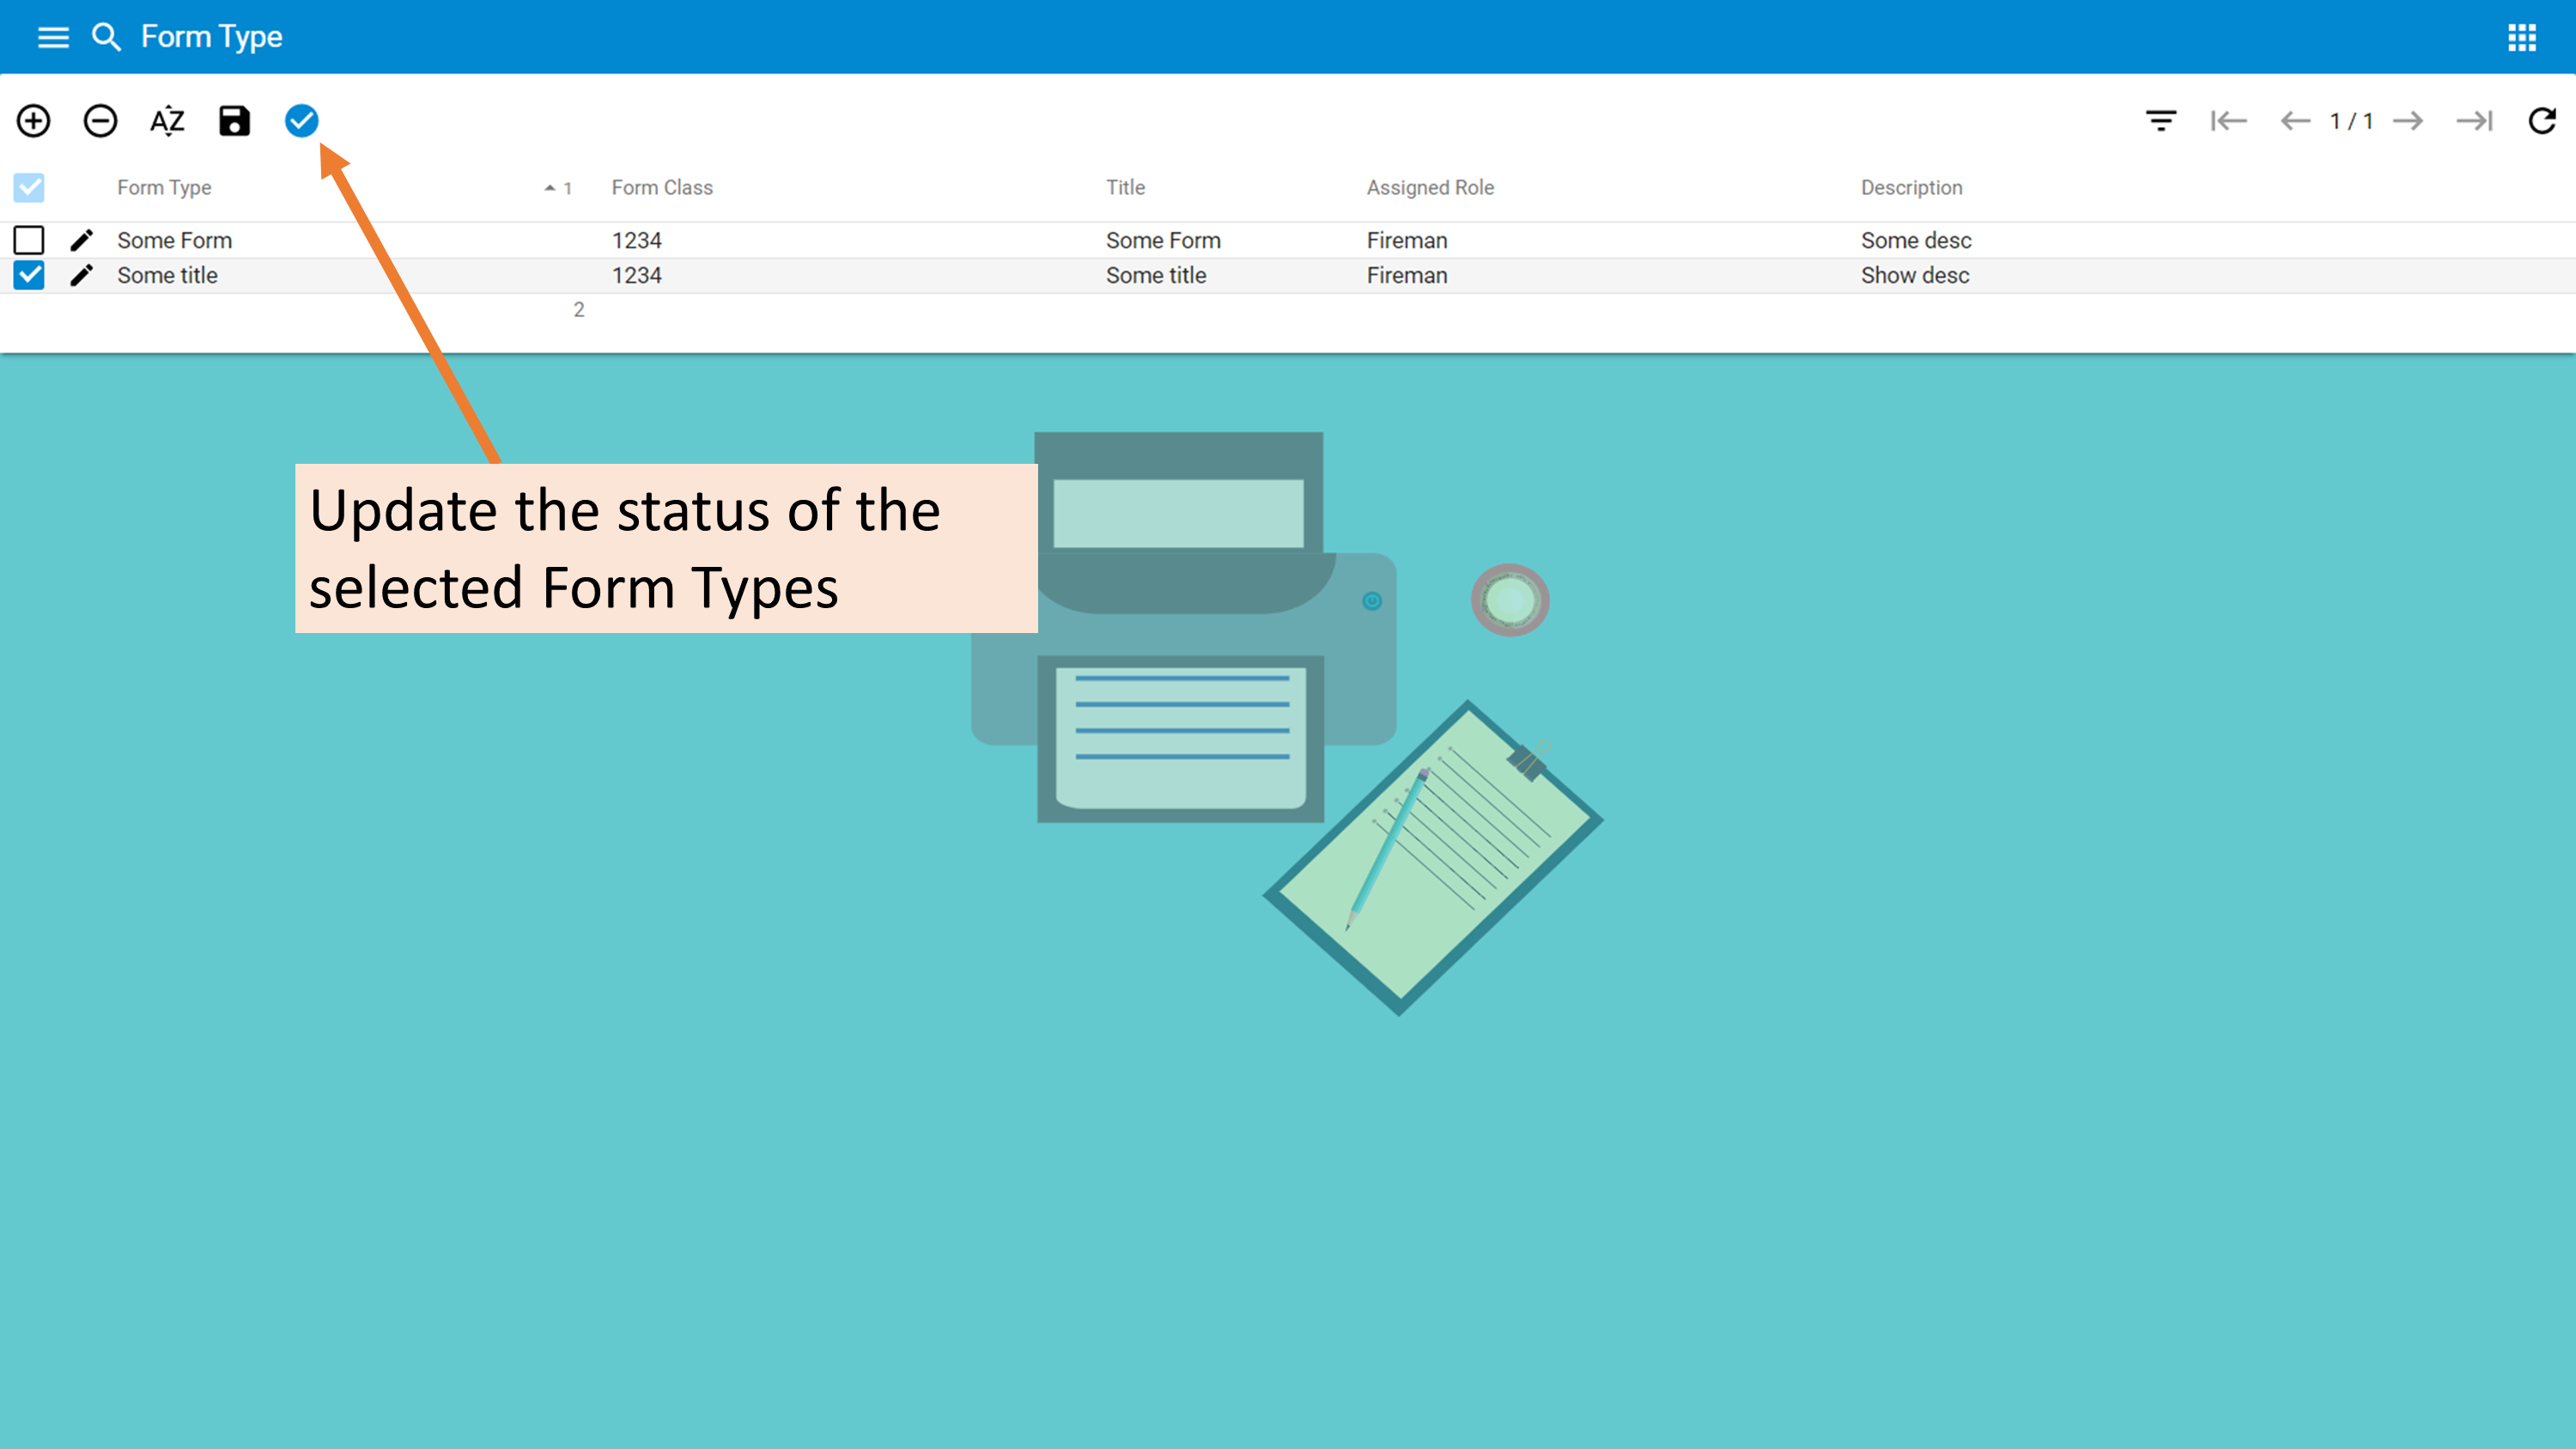
\includegraphics[width=0.95\linewidth]{sections/forms/images/form_type-batch_update.png}
\caption{Form Type Batch Update.}\label{sections/forms/images/form_type-batch_update}
\end{figure}


\newpage

\subsection{Form Class}
Form Class is a tool to create the Forms that will be deployed for everyday use. For example, a worker Andriy created the Form that can be approved by other employees. The Form has the autogenerated name, Status, Date created and Person that is responsible for this form.

\begin{figure}[!htbp]
\centering
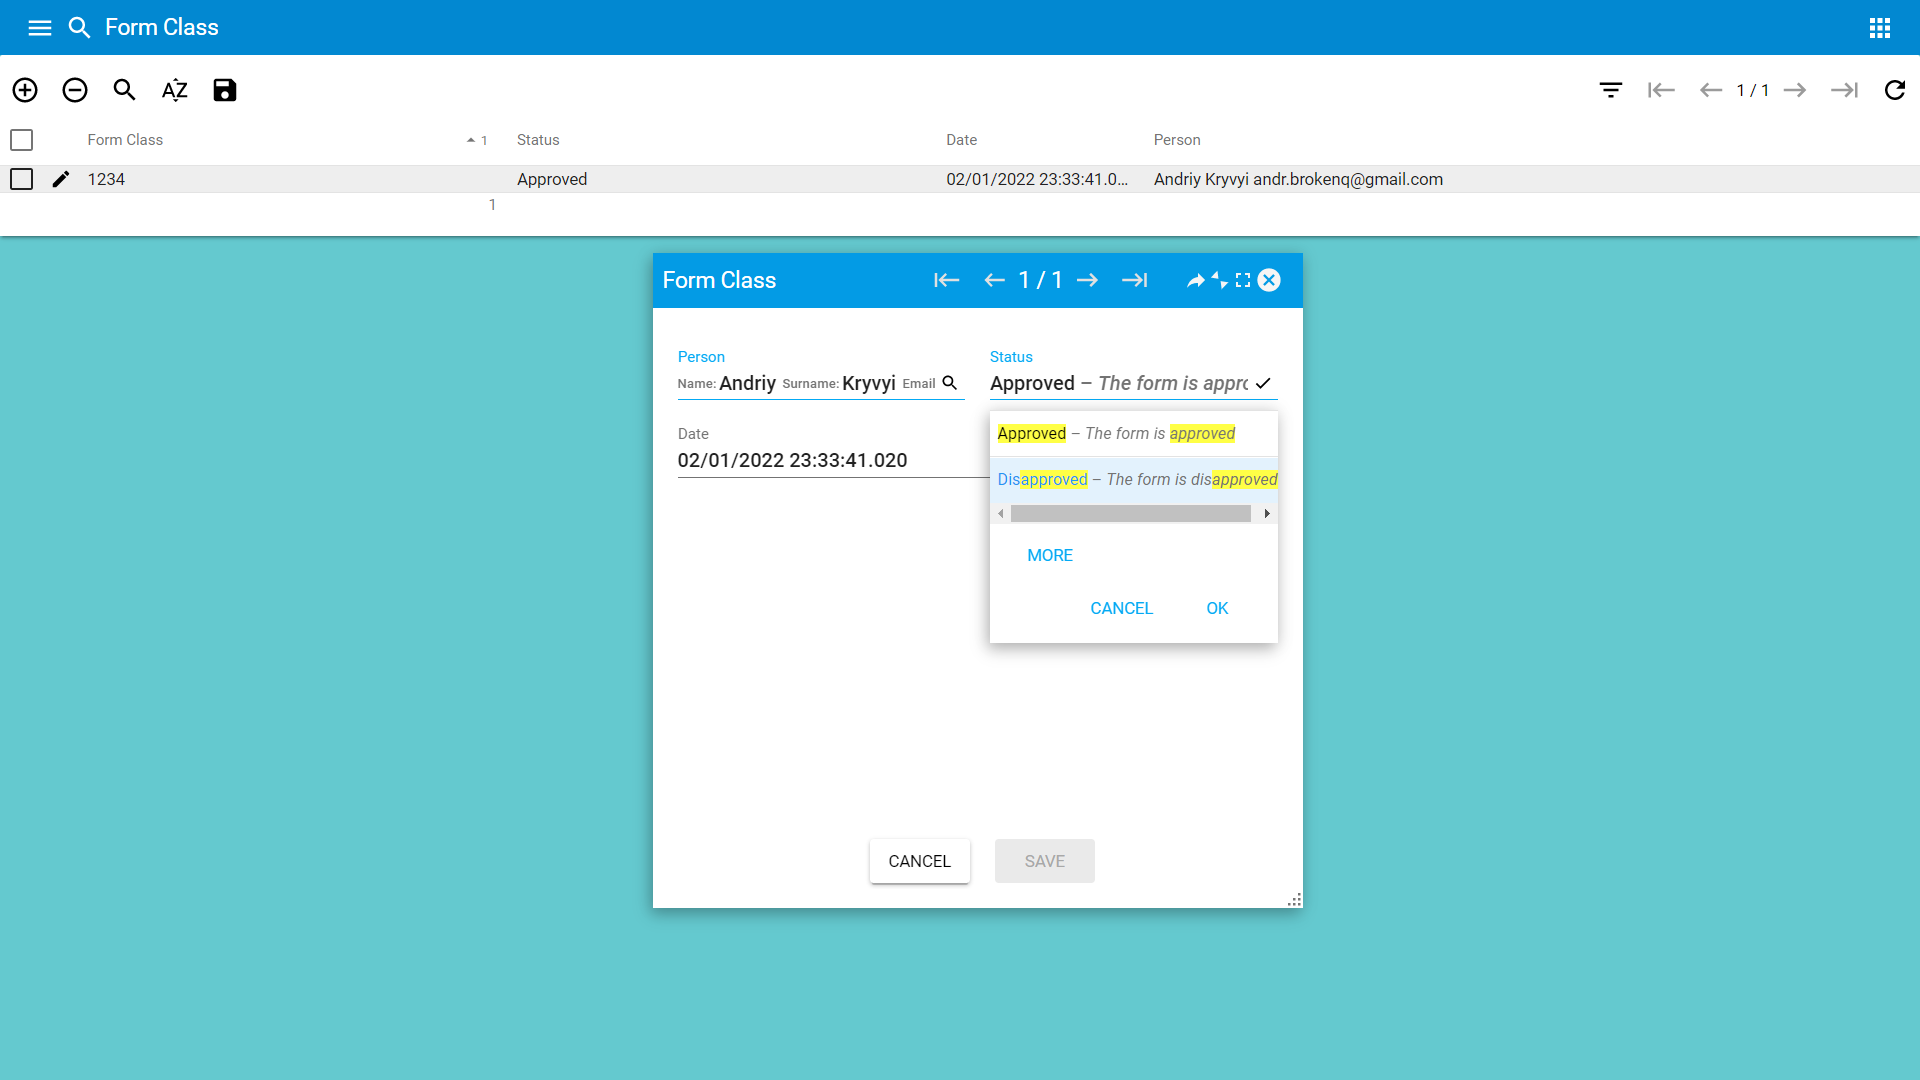
\includegraphics[width=0.95\linewidth]{sections/forms/images/form_class_master.png}
\caption{Form creation.}\label{sections/forms/images/form_class_master}
\end{figure}

Form search query can be used to filter the existing forms, and then delete or update them. 
\begin{figure}[!htbp]
\centering
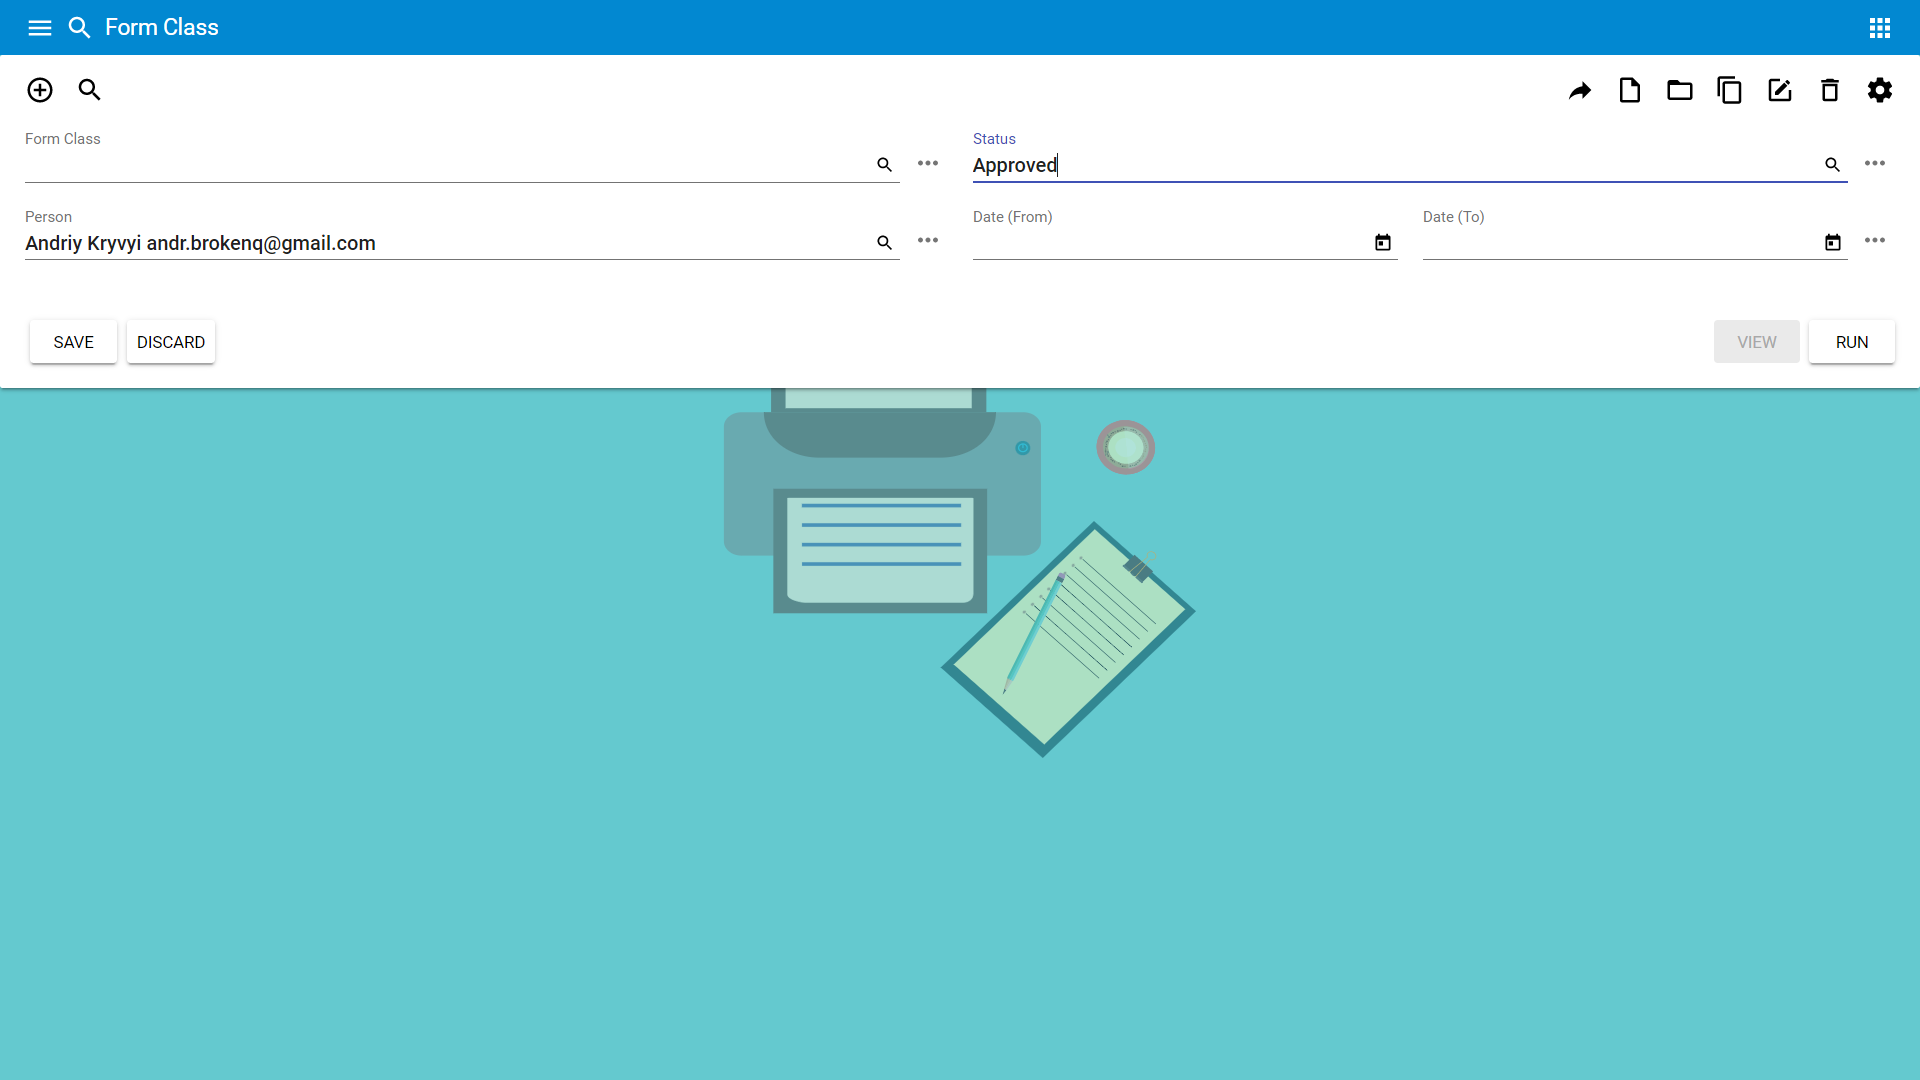
\includegraphics[width=0.95\linewidth]{sections/forms/images/form_class_centre.png}
\caption{Form search query.}\label{sections/forms/images/form_class_centre}
\end{figure}
\newpage

